\documentclass[a4paper]{article}
\usepackage{cmap}
\usepackage[utf8]{inputenc}
\usepackage[T2A]{fontenc}
\usepackage[english,russian]{babel} 
\usepackage[left=15mm, top=15mm, right=15mm, bottom=30mm, nohead, nofoot]{geometry}
\usepackage{blindtext}  % рыба-текст
\usepackage{graphicx}  % изображения
\usepackage{float} % плавающие объекты
\usepackage{wrapfig}  % изображения
\usepackage{tikz} % графика
\usepackage{mdframed} % рамки
\usepackage{xcolor} % определение цветов
\usepackage{nicefrac} % красивые дроби
\usepackage{cancel} % сокращение
\usepackage{amsmath,amsfonts,amssymb} % математический пакет
\usepackage{hyperref}  % гиперссылки
\usepackage{fancybox,fancyhdr} % хедер и футер
\usepackage{listings} % код
\usepackage[skip=2pt]{caption} % расстояние между подписью и картинкой
\pagestyle{fancy}
\fancyhf{}
\fancyhead[L]{Практическая работа №3}
\fancyhead[R]{\textit{Бифуркации}}
\fancyfoot[C]{\thepage}
\headsep=4mm
\footskip=13mm
\setlength{\parindent}{0em}
\setlength{\parsep}{0em}
\setlength{\headheight}{12pt}
\setlength{\topmargin}{-38pt}
\setlength{\arraycolsep}{2pt}

\definecolor{urlcolor}{HTML}{3454D1}
\definecolor{linkcolor}{HTML}{3454D1}
\hypersetup{
    pdfstartview=FitH,
    linkcolor=linkcolor,
    urlcolor=urlcolor,
    colorlinks=true,
    pdftitle={Практическая работа №3},
    pdfauthor={Овчинников П.А.}
}

\definecolor{strings}{rgb}{0,0.6,0}
\definecolor{comments}{rgb}{0,0.3,0}
\definecolor{numbers}{rgb}{0.5,0.5,0.5}
\definecolor{keywords}{rgb}{0.09,0.61,0.95}
\definecolor{background}{rgb}{0.97,0.97,0.97}
\lstdefinestyle{codestyle}{
    backgroundcolor=\color{background},
    commentstyle=\color{comments},
    keywordstyle=\color{keywords},
    stringstyle=\color{strings},
    numberstyle=\tiny\color{numbers},
    basicstyle=\ttfamily\footnotesize,
    breakatwhitespace=false,
    breaklines=true,
    captionpos=b,
    inputencoding=utf8,
    keepspaces=true,
    numbers=left,
    numbersep=5pt,
    showspaces=false,
    showstringspaces=false,
    showtabs=false,
    tabsize=2,
    extendedchars=true,
    literate=
    {а}{{\cyra}}1
    {б}{{\cyrb}}1
    {в}{{\cyrv}}1
    {г}{{\cyrg}}1
    {д}{{\cyrd}}1
    {е}{{\cyre}}1
    {ж}{{\cyrzh}}1
    {з}{{\cyrz}}1
    {и}{{\cyri}}1
    {й}{{\cyrishrt}}1
    {к}{{\cyrk}}1
    {л}{{\cyrl}}1
    {м}{{\cyrm}}1
    {н}{{\cyrn}}1
    {о}{{\cyro}}1
    {п}{{\cyrp}}1
    {р}{{\cyrr}}1
    {с}{{\cyrs}}1
    {т}{{\cyrt}}1
    {у}{{\cyru}}1
    {ф}{{\cyrf}}1
    {х}{{\cyrh}}1
    {ц}{{\cyrc}}1
    {ч}{{\cyrch}}1
    {ш}{{\cyrsh}}1
    {щ}{{\cyrshch}}1
    {ъ}{{\cyrhrdsn}}1
    {ы}{{\cyrery}}1
    {ь}{{\cyrsftsn}}1
    {э}{{\cyrerev}}1
    {ю}{{\cyryu}}1
    {я}{{\cyrya}}1
    {А}{{\CYRA}}1
    {Б}{{\CYRB}}1
    {В}{{\CYRV}}1
    {Г}{{\CYRG}}1
    {Д}{{\CYR96}}1
    {Е}{{\CYRE}}1
    {Ж}{{\CYRZH}}1
    {З}{{\CYRZ}}1
    {И}{{\CYRI}}1
    {Й}{{\CYRISHRT}}1
    {К}{{\CYRK}}1
    {Л}{{\CYRL}}1
    {М}{{\CYRM}}1
    {Н}{{\CYRN}}1
    {О}{{\CYRO}}1
    {П}{{\CYRP}}1
    {Р}{{\CYRR}}1
    {С}{{\CYRS}}1
    {Т}{{\CYRT}}1
    {У}{{\CYRU}}1
    {Ф}{{\CYRF}}1
    {Х}{{\CYRH}}1
    {Ц}{{\CYRC}}1
    {Ч}{{\CYRCH}}1
    {Ш}{{\CYRSH}}1
    {Щ}{{\CYRSHCH}}1
    {Ъ}{{\CYRHRDSN}}1
    {Ы}{{\CYRERY}}1
    {Ь}{{\CYRSFTSN}}1
    {Э}{{\CYREREV}}1
    {Ю}{{\CYRYU}}1
    {Я}{{\CYRYA}}1
}
\lstset{style=codestyle}

\addto\captionsrussian{
  \renewcommand{\contentsname}
    {\centering Содержание}
}
\newcommand{\addsection}[1]{
    \phantomsection
    \addcontentsline{toc}{section}{#1}
    \section*{\centering #1}
}
\newcommand{\addsubsection}[1]{
    \phantomsection
    \addcontentsline{toc}{subsection}{#1}
    \subsection*{\centering #1}
}
\newcommand{\addsubsubsection}[1]{
    \phantomsection
    \addcontentsline{toc}{subsubsection}{#1}
    \subsubsection*{\centering #1}
}

\newmdenv[
    leftmargin = 0.5em,
    skipabove = 0.5em,
    skipbelow = 0.5em,
    linewidth = 1pt,
    rightline = false,
    topline = false,
    bottomline = false
]{quotebox}

\newlength{\tempheight}
\newcommand{\Let}{
\mathbin{\text{\settoheight{\tempheight}{\mathstrut}\raisebox{0.4\pgflinewidth}{
\tikz[baseline=0.5ex,line cap=round,line join=round] \draw (0,0) --++ (0.3em,0) --++ (0,2.3ex) --++ (-0.3em,0);
}}}}
\newcommand*\squared[1]{\tikz[baseline=(char.base)]{
            \node[shape=rectangle,draw,inner sep=4pt] (char) {#1};}}
\newcommand*\msquared[1]{\tikz[baseline=(char.base)]{
            \node[shape=rectangle,draw,inner sep=4pt] (char) {$\displaystyle #1$};}}
\newcommand\argmax[1]{\underset{#1}{\text{argmax}}}
\renewcommand\max[1]{\underset{#1}{\text{max}}}
\newcommand{\at}{\biggr\rvert}
\newcommand{\shiftright}[3]{\makebox[#2][r]{\makebox[#1][l]{#3}}}
\newcommand{\e}{\;\text{e}}
\let\oldint\int
\def\int{\oldint\limits}
\DeclareRobustCommand{\divby}{%
  \mathrel{\vbox{\baselineskip.65ex\lineskiplimit0pt\hbox{.}\hbox{.}\hbox{.}}}%
}

\newcommand\NB{\textbf{N\kern-0.32em\textcolor{red}{B}}}

\begin{document}
\begin{titlepage}
    \begin{center}
    \includegraphics[width=0.18\textwidth]{~/Изображения/itmo_logo.png}\\[10pt]
        Федеральное государственное автономное образовательное \\ учреждение высшего образования \\[6pt]
        САНКТ-ПЕТЕРБУРГСКИЙ НАЦИОНАЛЬНЫЙ \\ ИССЛЕДОВАТЕЛЬСКИЙ УНИВЕРСИТЕТ ИТМО \\[16pt]
        Факультет систем управления и робототехники \vfill
        {\large Практическая работа №3} \\[0.5em]
        {\large \textbf{\MakeUppercase{Бифуркации}}}\\[0.5em]
        Вариант №4
    \end{center}\vfill
    \begin{flushright}
        \begin{minipage}{0.3\textwidth}
            Студенты:\\339308, Дьячихин Д.Н. (1.1) \\ 368606, Овчинников П.А. (1.2) \\ 368731, Румянцев А.А. (1.2)\\[0.5em]
            Преподаватель: Семёнов Д.М.
        \end{minipage}
    \end{flushright}\vfill
    \begin{center}
        {\small Санкт-Петербург \\ 2024}
    \end{center}
\end{titlepage}
\setcounter{page}{2}
\addsection{Задание}
Дана нелинейная система, согласно варианту:
$$\begin{cases}
    \dot{x}_1 = x_2, \\
    \dot{x}_2 = -x_1 - (x_1^2 - r)x_2;
\end{cases}$$
\begin{itemize}
    \item Найти возможные бифуркации в системе. Определить тип положений равновесия для всех значений бифуркационного параметра $r$.
    \item Построить фазовые портреты систем при различных бифуркационных параметрах.
\end{itemize}
\addsection{Выполнение работы}
Рассмотрим первый пункт. Для начала найдём положения равновесия системы:
$$\begin{cases}
    x_2 = 0, \\
    -x_1 - (x_1^2 - r)x_2 = 0
\end{cases} \quad\Rightarrow \quad \begin{cases}
    x_1 = 0, \\
    x_2 = 0. \\
\end{cases}$$
Похоже, что система имеет только одно положение равновесия в точке $(0, 0)$.\\[0.5em]
Теперь линеаризуем систему вблизи точек равновесия. Для этого найдём матрицу Якоби:
$$\dot{x} = Jx,\quad J = \begin{bmatrix}
    \nicefrac{\partial \dot{x}_1}{\partial x_1} & \nicefrac{\partial \dot{x}_1}{\partial x_2} \\
    \nicefrac{\partial \dot{x}_2}{\partial x_1} & \nicefrac{\partial \dot{x}_2}{\partial x_2}
\end{bmatrix} = \left.\begin{bmatrix}
    0 & 1 \\
    -1 - 2x_1x_2 & -x_1^2 + r
\end{bmatrix}\right|_{(0, 0)} = \begin{bmatrix}
    0 & 1 \\
    -1 & r
\end{bmatrix}.$$
А теперь найдём собственные значения матрицы:
$$|\lambda I - J| = \begin{vmatrix}
    \lambda & -1 \\
    1 & \lambda - r
\end{vmatrix} = 0 \quad\Rightarrow\quad \lambda^2-\lambda r + 1 = 0 \quad\Rightarrow\quad \lambda_{1,2} = \frac{r \pm \sqrt{r^2-4}}{2} \quad\Rightarrow\quad \lambda_{1,2} = \frac{r}{2} \pm \sqrt{\left( \frac{r}{2} \right)^2-1}.$$
В случае положительных значений $r\geqslant2$ собственные значения будут также положительными и вещественными. В случае отрицательных значений $r \leqslant -2$ собственные значения будут отрицательными и тоже вещественными. Собственные значения будут комплексными для $-2 < r < 2$, причём для $r = 0$ собственные значения будут чисто мнимыми. Это означает, что:
\begin{itemize}
    \item для $r \in \left( -\infty, -2\right]$ система имеет устойчивый узел, т.к. $\lambda_{1,2} < 0$ и $\Im(\lambda_{1,2}) = 0$;
    \item для $r \in \left( -2, 0\right)$ система имеет устойчивый фокус, т.к. $\Re(\lambda_{1,2}) < 0$ и $\Im(\lambda_{1,2}) \neq 0$;
    \item для $r = 0$ система имеет центр, вращающийся по часовой стрелке, т.к. $\Re(\lambda_{1,2}) = 0$ и $\Im(\lambda_{1,2}) \neq 0$;
    \item для $r \in \left( 0, 2\right)$ система имеет неустойчивый фокус, т.к. $\Re(\lambda_{1,2}) > 0$ и $\Im(\lambda_{1,2}) \neq 0$;
    \item для $r \in \left[ 2, +\infty\right)$ система имеет неустойчивый узел, т.к. $\lambda_{1,2} > 0$ и $\Im(\lambda_{1,2}) = 0$.
\end{itemize}
\vspace{0.5em}
Теперь перейдём ко второму пункту. Построим фазовые портреты системы при различных значениях параметра $r$. Для этого напишем программу на языке Python, используя высокоуровневый модуль для построения фазовых траекторий \texttt{phaseportrait}. Код программы представлен в листинге \ref{code}.\\[0.5em]
Рассмотрим фазовые портреты системы при различных значениях параметра $r$:
\begin{figure}[H]
    \centering
    \begin{minipage}{0.395\textwidth}
        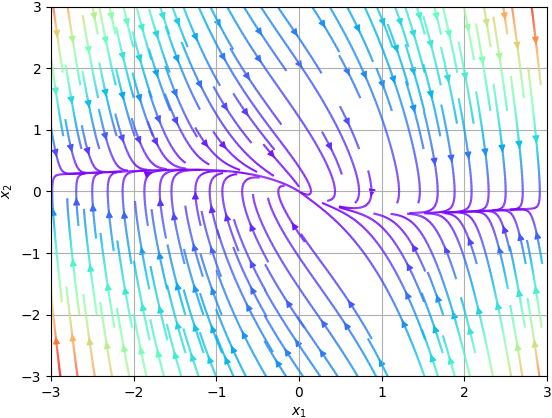
\includegraphics[width=\textwidth]{sources/r<=-2.png}
        \caption{$r \in \left( -\infty, -2\right]$}
    \end{minipage}
    \hspace{2em}
    \begin{minipage}{0.395\textwidth}
        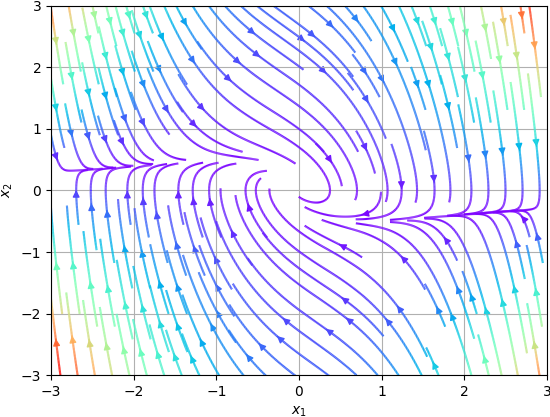
\includegraphics[width=\textwidth]{sources/-2<r<0.png}
        \caption{$r \in \left( -2, 0\right)$}
    \end{minipage}
\end{figure}
\begin{figure}[H]
    \centering
    \begin{minipage}{0.395\textwidth}
        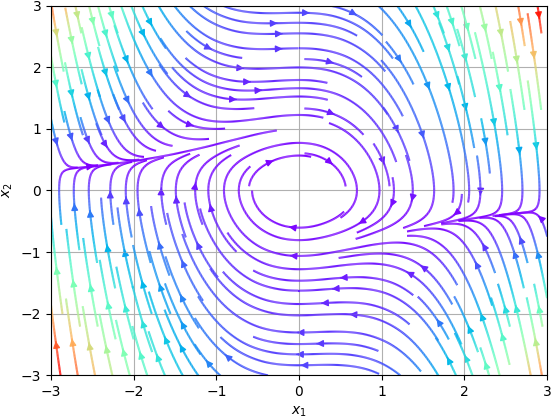
\includegraphics[width=\textwidth]{sources/r=0.png}
        \caption{$r = 0$}
    \end{minipage}
    \hspace{2em}
    \begin{minipage}{0.395\textwidth}
        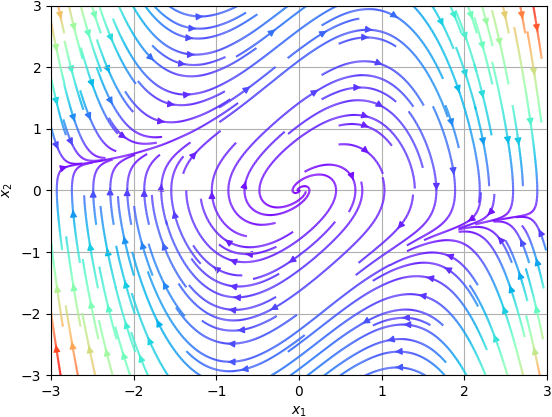
\includegraphics[width=\textwidth]{sources/0<r<2.png}
        \caption{$r \in \left( 0, 2\right)$}
    \end{minipage}
\end{figure}
\begin{figure}[H]
    \centering
    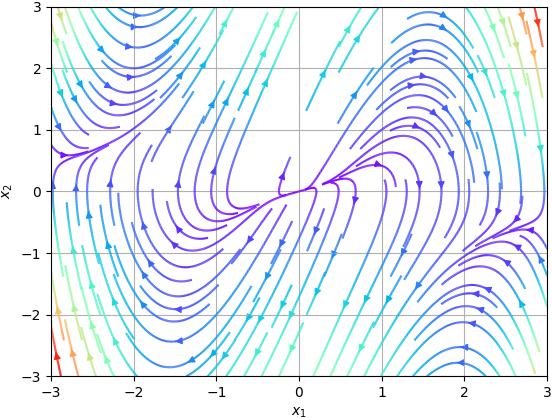
\includegraphics[width=0.395\textwidth]{sources/r>=2.png}
    \caption{$r \in \left[ 2, +\infty\right)$}
\end{figure}
\begin{lstlisting}[language=Python, caption=Код программы, label=code]
import os
try:
    from phaseportrait import PhasePortrait2D
except ImportError:
    os.system('pip install phaseportrait')
    from phaseportrait import PhasePortrait2D

r = 0  # значение r можно задать здесь
def df(x1, x2):
    return x2, -x1 - (x1 ** 2 - r) * x2


def render_pp(df, x_center, y_center):
    pp = PhasePortrait2D(df, [min(x_center, y_center) - 3, max(x_center, y_center) + 3], numba=True, Title='', xlabel='$x_1$', ylabel='$x_2$')
    fig, ax = pp.plot()
    ax.set_xlim(x_center - 3, x_center + 3)
    ax.set_ylim(y_center - 3, y_center + 3)
    ax.set_xticks(range(x_center - 3, x_center + 4))
    ax.set_yticks(range(y_center - 3, y_center + 4))
    fig.savefig(f'sources/{df.__name__}.png')

os.makedirs('sources', exist_ok=True)
render_pp(df, 0, 0)
print('Done!')
\end{lstlisting}
\addsection{Вывод}
В ходе выполнения практической работы мы научились искать положения равновесия системы и определять типы фазовых портретов системы. Также мы научились строить фазовые траектории программно, чтобы сверять результаты с теоретическими расчётами. Наши расчёты оказались верны и фазовые траектории определены корректно.
\end{document}